\scanpage{71}
Groupoïdes de \uline{Teichmüller}

1) Groupoïdes topologiques $\boxed{S\mathcal T_{\mathrm{top}}}$.
(\uline{groupoïde de Teichmüller spécial orienté topologique})

Objets : paires $(X,S)$
\[
\left|\begin{array}{l}
X\ \text{surface à bord compacte \uline{orientée}}\\
S\subset\partial X\quad\text{partie finie du bord}
\end{array}\right.
\]
Morphismes $(X,S)\longrightarrow(X',S')$ : classes d'isotopie d'isomorphismes

\deleted{\unsure{Trois}} \uline{Variantes}

$1^\circ)$ $S=\varnothing$ on écrit $\mathcal T_{\mathrm{top}}$ sous-groupoïde ouvert.
(\uline{groupoïde de T. \deleted{\unsure{orient}} orienté topologique})

$2^\circ)$ $\boxed{S\mathcal T_{\mathrm{top}}^\pm}$ mêmes objets, mais plus de flèches :
classes d'isotopie d'homéom. $(X,S)\xrightarrow{\sim}(X',S')$, ne respectant pas l'orientation nécessairement.

On a
\diagram{\begin{tikzcd}[ampersand replacement=\&,column sep=large]
S\mathcal T_{\mathrm{top}}^\pm \arrow[r,"\unsure{\chi}","\text{(signature)}"']
\& \deleted{\unsure{\mathfrak G}}\ \substack{\text{groupoïde \deleted{ponctuel}}\\
\text{défini par le groupe}\\
\pm1,\ \text{noté }[\pm1]}
\end{tikzcd}}
\unsure{le|la} \deleted{noyau} \deleted{est} (la catégorie fibre) est $S\mathcal T_{\mathrm{top}}$

$2^\circ)$ $(X,\Sigma,S)$, avec
\[
\left|\begin{array}{l}
X\ \text{compacte à bord orienté}\\
\Sigma\ \text{sous-variété \deleted{fermée} \inserted{compacte} de dim $1$}\\
\qquad\text{de }X\setminus\partial X\\
S\subset\Sigma\cup\partial X\quad\text{partie finie}
\end{array}\right.
\]
morphismes : classes d'isotopie d'homéom respectant l'orientation.
Notation $\mathcal T\deleted{\unsure{S}}\inserted{D}_{\mathrm{top}}$
($D$ initiale de dévissage \deleted{``\unsure{sauvage}''}) :
``\uline{groupoïde de Teichmüller orienté dévissé topologique}''.

\uline{NB}
\[
S\mathcal T_{\mathrm{top}}\subset S\mathcal TD_{\mathrm{top}}
\qquad
\substack{\text{imm. ouverte}\\(\deleted{\text{immersion pleine}})}
\]
\[
\substack{\Vert\\\text{sous groupoïde des objets tels que }\Sigma=\varnothing}
\]

$3^\circ)$ On définit de $=$ $\unsure{\mathcal TS_{\mathrm{top}}^\pm}$
(\uline{groupoïde de Teichmüller bi-orienté dévissé topologique})
\figure{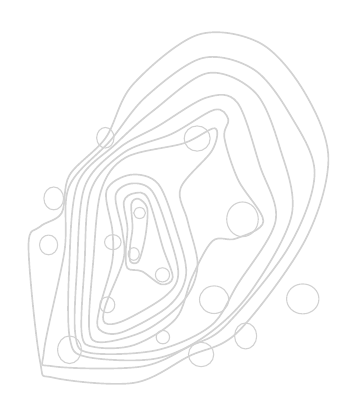
\begin{tikzpicture}[x=-.005cm,y=-.005cm,rotate=90]
\coordinate (a) at (878,350);
\coordinate (b) at (996,337);
\coordinate (c) at (1262,390);
\coordinate (d) at (724,481);
\coordinate (e) at (989,500);
\coordinate (f) at (915,568);
\coordinate (g) at (1019,553);
\coordinate (h) at (1148,486);
\coordinate (i) at (1072,626);
\coordinate (j) at (1230,627);
\coordinate (k) at (726,714);
\coordinate (l) at (931,829);
\coordinate (m) at (1135,757);
\coordinate (n) at (1274,724);
\coordinate (o) at (1227,837);
\coordinate (p) at (1133,982);
\draw[gray!35,line width=.6pt] plot[smooth cycle,tension=.55] coordinates {(724,482) (590,550) (463,715) (484,874) (608,986) (777,1047) (984,988) (1215,819) (1278,694) (1346,554) (1333,350) (1290,315) (1000,286) (950,315) (915,370) (819,390)};
\draw[gray!35,line width=.6pt] plot[smooth cycle,tension=.55] coordinates {(732,493) (620,584) (522,727) (551,858) (666,950) (814,1012) (1000,947) (1200,787) (1253,695) (1305,571) (1304,348) (1267,325) (1014,377) (848,389)};
\draw[gray!35,line width=.6pt] plot[smooth cycle,tension=.55] coordinates {(740,507) (655,603) (560,741) (609,861) (747,923) (919,954) (1116,849) (1227,735) (1285,606) (1280,433) (1234,391) (1063,389) (843,410)};
\draw[gray!35,line width=.6pt] plot[smooth cycle,tension=.55] coordinates {(751,515) (695,614) (622,738) (635,816) (795,873) (935,913) (1097,816) (1201,749) (1263,612) (1270,442) (1224,405) (1055,409) (850,428)};
\draw[gray!35,line width=.6pt] plot[smooth cycle,tension=.55] coordinates {(761,529) (714,650) (653,758) (677,793) (724,783) (831,818) (936,882) (980,812) (986,753) (1078,701) (1183,660) (1250,554) (1255,453) (1221,421) (1049,428) (858,444)};
\draw[gray!35,line width=.6pt] plot[smooth cycle,tension=.55] coordinates {(774,533) (738,680) (700,759) (756,752) (852,672) (936,690) (1049,715) (1137,680) (1213,583) (1243,471) (1209,440) (1041,450) (859,470)};
\draw[gray!35,line width=.6pt] plot[smooth cycle,tension=.55] coordinates {(858,484) (818,545) (841,615) (958,661) (1070,686) (1150,643) (1218,522) (1210,465) (1158,466) (1041,498) (961,499)};
\draw[gray!35,line width=.6pt] plot[smooth cycle,tension=.55] coordinates {(870,507) (840,548) (860,600) (968,642) (1071,666) (1127,632) (1188,528) (1194,480) (1151,481) (1033,527) (961,524)};
\draw[gray!35,line width=.6pt] plot[smooth cycle,tension=.55] coordinates {(886,528) (865,554) (878,589) (1003,627) (1078,652) (1096,623) (1063,574) (1055,537) (1010,533) (952,537)};
\draw[gray!35,line width=.6pt] plot[smooth cycle,tension=.55] coordinates {(892,547) (879,565) (902,587) (958,585) (1009,575) (1040,563) (1037,544) (997,544) (952,550)};
\draw[gray!35] (a) ellipse (29 and 25);
\draw[gray!35] (b) ellipse (25 and 23);
\draw[gray!35] (c) ellipse (35 and 30);
\draw[gray!35] (d) ellipse (26 and 22);
\draw[gray!35] (e) ellipse (19 and 21);
\draw[gray!35] (f) ellipse (14 and 15);
\draw[gray!35] (g) ellipse (16 and 14);
\draw[gray!35] (h) ellipse (20 and 19);
\draw[gray!35] (i) ellipse (18 and 18);
\draw[gray!35] (j) ellipse (17 and 17);
\draw[gray!35] (k) ellipse (32 and 33);
\draw[gray!35] (l) ellipse (44 and 40);
\draw[gray!35] (m) ellipse (35 and 37);
\draw[gray!35] (n) ellipse (31 and 32);
\draw[gray!35] (o) ellipse (33 and 28);
\draw[gray!35] (p) ellipse (38 and 41);\end{tikzpicture}}
\mspage{70}
